% Этот шаблон документа разработан в 2014 году
% Данилом Фёдоровых (danil@fedorovykh.ru) 
% для использования в курсе 
% <<Документы и презентации в \LaTeX>>, записанном НИУ ВШЭ
% для Coursera.org: http://coursera.org/course/latex .
% Исходная версия шаблона --- 
% https://www.writelatex.com/coursera/latex/2

\documentclass[../main.tex]{subfiles}

%%% Работа с русским языком
\usepackage{cmap}					% поиск в PDF
\usepackage{mathtext} 				% русские буквы в формулах
\usepackage[T2A]{fontenc}			% кодировка
\usepackage[utf8]{inputenc}			% кодировка исходного текста
\usepackage[english,russian]{babel}	% локализация и переносы

%%% Дополнительная работа с математикой
\usepackage{amsfonts,amssymb,amsthm,mathtools} % AMS
\usepackage{amsmath}
\usepackage{icomma} % "Умная" запятая: $0,2$ --- число, $0, 2$ --- перечисление

%% Номера формул
%\mathtoolsset{showonlyrefs=true} % Показывать номера только у тех формул, на которые есть \eqref{} в тексте.
%% Шрифты
\usepackage{euscript}	 % Шрифт Евклид
\usepackage{mathrsfs} % Красивый матшрифт

%% Свои команды
\DeclareMathOperator{\sgn}{\mathop{sgn}}

%% Перенос знаков в формулах (по Львовскому)
\newcommand*{\hm}[1]{#1\nobreak\discretionary{}
	{\hbox{$\mathsurround=0pt #1$}}{}}

%%% Работа с картинками
\usepackage{graphicx}  % Для вставки рисунков
\graphicspath{{images/1/}{images/2/}{{images/4/}}}  % папки с картинками
\setlength\fboxsep{3pt} % Отступ рамки \fbox{} от рисунка
\setlength\fboxrule{1pt} % Толщина линий рамки \fbox{}
\usepackage{wrapfig} % Обтекание рисунков и таблиц текстом

%%% Работа с таблицами
\usepackage{array,tabularx,tabulary,booktabs} % Дополнительная работа с таблицами
\usepackage{longtable}  % Длинные таблицы
\usepackage{multirow} % Слияние строк в таблице


\usepackage{indentfirst}
\usepackage{hyperref}
\usepackage{booktabs}
\usepackage{float}
\usepackage[table]{xcolor}

% код в matlab
\usepackage{matlab-prettifier}
\usepackage{listings,lstautogobble}
\lstset{autogobble=true}



\begin{document} % конец преамбулы, начало документа
	
	В данной главе будет реализована одна вариация генетического алгоритма, которая затем будет протестирована на нескольких задачах. 
	
	\subsection{Описание генетического алгоритма}
	
	Для начала кратко опишем генетический алгоритм: данная процедура используется для решения задачи минимизации некоторой функции $f: \mathbb{R}^n \rightarrow \mathbb{R}$ на некотором множестве $D \subseteq \mathbb{R}^n$. Также предполагается, что она неотрицательная, иначе говоря $f(x) \geqslant 0 \text{ }\forall x \in D$. 
	
	В рамках алгоритма генами будут называться вектора переменных, то есть точки $x \in D$. Хромосомами будут называться компоненты данного вектора. 
	
	Идея алгоритма состоит в создании некоторой популяции генов, которая будет постепенно эволюционировать и находить все лучшее приближение минимума $f(x)$. Размер популяции $M$, количество итераций $L$ и заменяемых генов $M_c$ задается исследователем.  Опишем основные шаги рассматриваемой вариации генетического алгоритма:
	
	\begin{enumerate}
		\item Генерация популяции генов случайным образом.
		\item Подсчет функции приспособленности гена $fit(x) = \frac{1}{1 + f(x)}$ и сортировка популяции по убыванию значений приспособленности.
		\item Замена каждой особи с номером $m \in [2, M - M_c]$ на результат ее скрещивания со случайной особью в пуле. 
		
		Скрещивание двух генов $x, y \in \mathbb{R}^n$ подразумевает создание нового гена $z$, где каждая хромосома $z_i$ будет взята случайно из множества $\{x_i, y_i\}$, причем $\mathbb{P}(z_i = x_i) = \frac{fit(x)}{fit(x) + fit(y)}$.
		
		\item Замена $M_c$ наименее приспособленных особей случайно сгенерированными генами.
		\item Возврат к шагу 2, если количество итераций не достигло $L$.
		
	\end{enumerate}

	Заметим, что лучшая особь на каждой итерации не изменяется, поэтому алгоритм гарантированно не ухудшает уже найденное приближение. Иначе говоря, последовательность значений функции будет монотонно(нестрого) убывать. Если $f(x)$ -- ограничена на множестве $D$, то по теореме Вейерштрасса вышеописанная последовательность будет иметь предел.
	
	Далее рассмотрим применение генетического алгоритма на нескольких задачах.
	
	\subsection{Минимизация числовой функции}
	
	Пусть 
	\[f(x) = \sum_{k=1}^{n}x_k^2 (1 + |\sin{(100x_k)}|)\]
	
	Требуется минимизировать данную функцию на множестве $D = [-10, 10]^n$. Нетрудно видеть, что глобальным минимумом является нулевой вектор размера $n$. Однако градиентными методами данную задачу решить представляется очень сложным ввиду большого количества локальных минимумов. Подтверждением этого тезиса является график функции для $n=1$.
	
	
	\begin{figure}[H]
		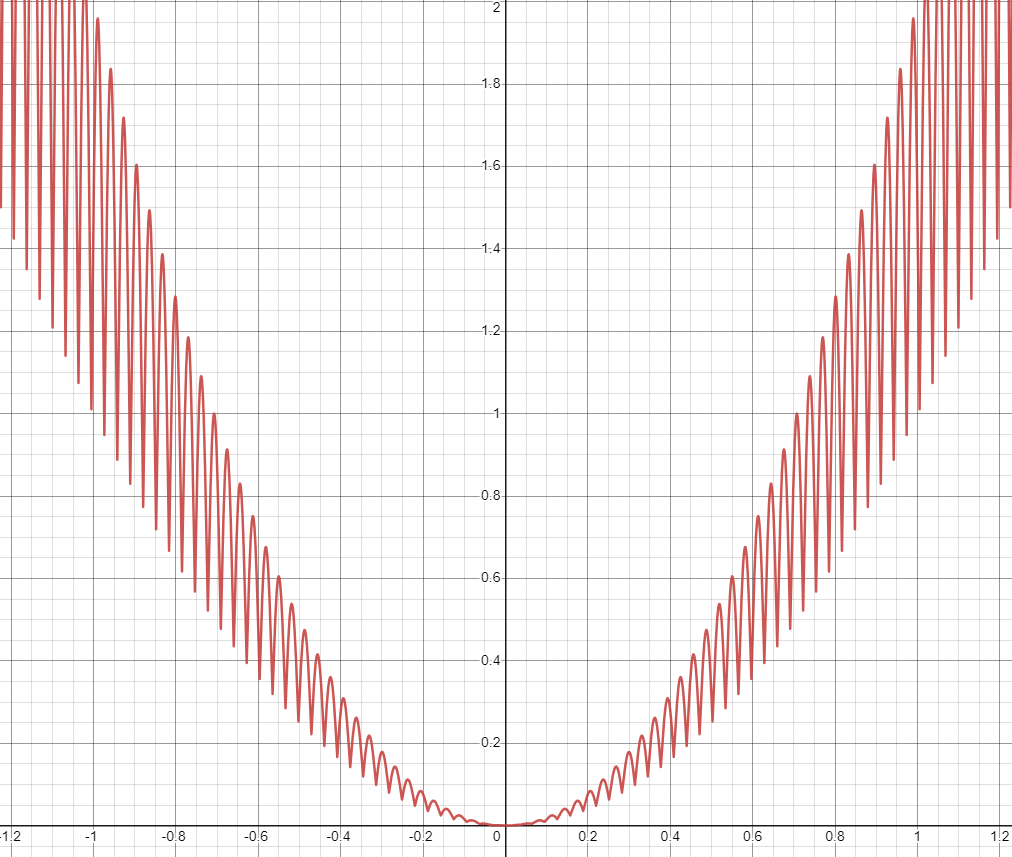
\includegraphics[width = \textwidth]{gen_1.png}{}
		\caption{График функции $f(x) = x^2 (1 + |\sin(100x)|)$}
		\label{fig: gen_alg_test_1}
	\end{figure}
	
	
	
	
	Рассмотрим случай $n=5$. Сначала реализуем расчет значений функции $f(x)$ в MATLAB: 
	
	\begin{lstlisting}[
		frame=single,
		numbers=left,
		style=Matlab-Pyglike]
		function [y] = gen_alg_test_1(X)
		dim = size(X, 2);
		y = 0;
		for i = 1:dim
		  y = y + X(:, i).^2 .* (1 + abs(sin(100 * X(:, i))));
		end		
	\end{lstlisting}

	Далее напишем код генетического алгоритма в соответствии с вышеописанными шагами для случая $n=5$. Генерация гена будет происходить из равномерного распределения на множестве $[-10, 10]^5$.
	
	\begin{lstlisting}[
		frame=single,
		numbers=left,
		style=Matlab-Pyglike]
		function [y_min, x_min] = gen_alg_unif(f, D, M, M_c, L) 
		dim = size(D, 1);
		X = zeros(M, dim);
		for i = 1:dim
		  x_lower = D(i, 1);
		  x_upper = D(i, 2);
		  X(:, i) = unifrnd(x_lower, x_upper, M, 1);
		end
		for t = 1:L
		  fit = ones(M, 1) ./ (1 + f(X));
		  X = [fit X];
		  X = sortrows(X, 1, "descend");
		  fit = X(:, 1);
		  X = X(:, 2:(dim + 1));
		  male_idx = 2:M - M_c;
		  female_idx = randsample(1:length(M), M - M_c - 1, true);
		  male = X(male_idx, :);
		  female = X(female_idx, :);
		  child_male_gen_ind = zeros(M - M_c - 1, dim);
		  male_proba = fit(male_idx) / (fit(male_idx) + fit(female_idx));
		  for i = 1:M - M_c - 1
			  child_male_gen_ind(i, :) = binornd(1, male_proba(i), 1, dim);
		  end
		  X = male .* child_male_gen_ind + female .* (1 - child_male_gen_ind);
		  replace_ind = (M - M_c + 1):M;
		  for i = 1:dim
			  x_lower = D(i, 1);
			  x_upper = D(i, 2);
			  X(replace_ind, i) = unifrnd(x_lower, x_upper, M_c, 1);
		  end
		end
		x_min = X(1, :);
		y_min = f(x_min);
	\end{lstlisting}
	

	Зафиксируем параметры алгоритма: $M = 1000, M_c = 200, L = 100$. В результате запуска получим:
	
	\begin{lstlisting}[
		frame=single,
		numbers=left,
		style=Matlab-Pyglike]
		>> [y_min, x_min] = gen_alg_unif(@gen_alg_test_1, repmat([-10, 10], 5, 1), 1000, 300, 100)
		
		y_min =
		
		0
		
		
		x_min =
		
		0     0     0     0     0	
	\end{lstlisting}

	Видно, что алгоритм нашел глобальный минимум, причем время исполнения не превышает одной секунды.
	
	\subsection{Дискретная задача}
	
	Перейдем к следующей задаче -- имеется множество $A = \{1, 2, \dots, n\}$, которое необходимо разбить на два непересекающихся множества $K_1$ и $K_2$ так, чтобы 
	
	\[H(K_1, K_2) =  \left|\sum_{a_k \in K_1}a_k - \sum_{a_m \in K_2}a_m \right|\]
	
	была минимальна. Причем $K_1 \cup K_2 = A, K_1 \cap K_2 = \varnothing$.
	
	Известно, что данная задача не решается точно за полиномиальное время -- воспользуемся генетическим алгоритмом для нахождения приближенного решения.
	
	Заметим, что разбиение $A$ взаимно-однозначно задается характеристическим вектором множества $K_1$, то есть вектором $x = \{\mathbb{I}\{i \in K_1\}\}_{i=1}^n$. Тогда вышеописанная задача сводится к минимизации  следующей функции 
	\[\begin{aligned}
		f(x) &= \left|\sum_{k=1}^{n}k \cdot \mathbb{I}\{x_k = 1\}  - \sum_{k=1}^{n}k \cdot \mathbb{I}\{x_k = 0\} \right| = \left|\sum_{k=1}^{n}k \cdot (\mathbb{I}\{x_k = 1\}  -\mathbb{I}\{x_k = 0\})\right| \\
		&\text{, где }x \in \{0, 1\}^n \\
	\end{aligned}\]
	
	Решим эту задачу, используя MATLAB. Реализация функции $f(x)$ будет иметь вид:
	
	\begin{lstlisting}[
		frame=single,
		numbers=left,
		style=Matlab-Pyglike]
		function [y] = gen_alg_test_2(X)
		dim = size(X, 2);
		start = 1;
		stop = start + dim - 1;
		A = repmat(start:stop, size(X, 1), 1);
		
		Z = zeros(size(X, 1), dim);
		mask_0 = X == 0;
		Z(mask_0) = A(mask_0);
		sum_0 = sum(Z, 2);
		
		Z = zeros(size(X, 1), dim);
		mask_1 = X == 1;
		Z(mask_1) = A(mask_1);
		sum_1 = sum(Z, 2);
		
		y = abs(sum_1 - sum_0);	
	\end{lstlisting}

	Генетический алгоритм будет применяться аналогично предыдущей задаче, однако теперь для создания случайного гена каждая хромосома будет независимо генерироваться из распределения Бернулли с параметром $p = \frac{1}{2}$. Тогда код генетического алгоритма будет следующим:
	
		\begin{lstlisting}[
		frame=single,
		numbers=left,
		style=Matlab-Pyglike]
		function [y_min, x_min] = gen_alg_bern(f, dim, M, M_c, L) 
		X = zeros(M, dim);
		X = binornd(1, 0.5, M, dim);
		for t = 1:L
		  fit = ones(M, 1) ./ (1 + f(X));
		  X = [fit X];
	 	 X = sortrows(X, 1, "descend");
		  fit = X(:, 1);
		  X = X(:, 2:(dim + 1));
		  male_idx = 2:M - M_c;
		  female_idx = randsample(1:length(M), M - M_c - 1, true);
		  male = X(male_idx, :);
		  female = X(female_idx, :);
		  child_male_gen_ind = zeros(M - M_c - 1, dim);
		  male_proba = fit(male_idx) / (fit(male_idx) + fit(female_idx));
		  for i = 1:M - M_c - 1
		    child_male_gen_ind(i, :) = binornd(1, male_proba(i), 1, dim);
		  end
		  X = male .* child_male_gen_ind + female .* (1 - child_male_gen_ind);
		  replace_ind = (M - M_c + 1):M;
		  X(replace_ind, :) = binornd(1, 0.5, M_c, dim);
		end
		x_min = X(1, :);
		y_min = f(x_min);
	\end{lstlisting}

	Оставим параметры алгоритма фиксированными на прежнем уровне и запустим оптимизацию для $n=100, n=1000, n=10000$.
	
	 	\begin{lstlisting}[
	 	frame=single,
	 	numbers=left,
	 	style=Matlab-Pyglike]
	 	>> [y_min, ~] = gen_alg_bern(@gen_alg_test_2, 100, 1000, 300, 100)
	 	
	 	y_min =
	 	
	 	0
	 	
	 	>> [y_min, ~] = gen_alg_bern(@gen_alg_test_2, 1000, 1000, 300, 100)
	 	
	 	y_min =
	 	
	 	0
	 	
	 	
	 	>> [y_min, ~] = gen_alg_bern(@gen_alg_test_2, 10000, 1000, 300, 100)
	 	
	 	y_min =
	 	
	 	22
	 	
	 \end{lstlisting}
 
 	Заметим, что при $n=100$ и $n=1000$ генетический алгоритм нашел оптимальное разбиение исходного множества на два подмножества с одинаковой суммой. При $n=10000$ суммы уже получились не одинаковыми, однако значение целевой функции оказалось относительно близким к нулю.
 	
 	\subsection{Линейное программирование}
 	
 	Задача линейного программирования заключается в минимизации линейной функции при условии ограничений-равенств и ограничений-неравенств, где функции ограничения имеют линейный вид. Кроме того, на некоторые переменные может быть наложено ограничение целочисленности и нахождение на некотором отрезке. Таким образом, данная задача будет иметь следующий вид
 	
 	\[\left\{\begin{aligned}
 		f(x) &= c^T x \rightarrow \underset{x \in \mathbb{R}^n}{\min} \\ 
 		Ax &\leqslant b \\
 		A_{eq} x &= b_{eq} \\
 		lb_i &\leqslant x_i \leqslant ub_i \text{ } \forall i \in J \\
 		x_i &\in \mathbb{Z}  \text{ }  \forall i \in Z\\
 	\end{aligned}\right.\]
 	, где $A, A_{eq} \in Mat_{m \text{ } n}(\mathbb{R})$; $b, b_{eq} \in \mathbb{R}^m$; $c \in \mathbb{R}^n$; $J, Z \subseteq \{1, 2, \dots, n\}$; $lb_i, ub_i \in \mathbb{R} \text{ } \forall i \in J$
 	
 	Теперь от данной общей постановки перейдем к более узкой, где нет ограничений-равенств, ограничений на целочисленность, верхних границ значений переменных. Также будем рассматривать только неотрицательные значения переменных и параметров задачи. Кроме того, теперь задача будет заключаться в максимизации целевой функции. То есть
 	
 	\[\left\{\begin{aligned}
 		f(x) &= c^T x \rightarrow \underset{x \in \mathbb{R}^n}{\max} \\ 
 		Ax &\leqslant b \\
		x_i &\geqslant 0  \text{ } \forall i \in  \{1, 2, \dots, n\} \\
 		x_i &\in \mathbb{Z}  \text{ }  \forall i \in Z\\
 	\end{aligned}\right.\]
 	, где $A \in Mat_{m \text{ } n}(\mathbb{R}_+)$; $b \in \mathbb{R}_+^m$; $c \in \mathbb{R}_+^n$; $Z \subseteq \{1, 2, \dots, n\}$;
 	
 	Данная задача чаще всего решается симплекс-методом, однако генетический алгоритм к ней так же применим -- реализуем его в MATLAB.
 	
 	Заметим, что основная часть этого алгоритма уже была реализована в вышеописанных задачах, поэтому необходимо лишь адаптировать эти наработки под задачу линейного программирования. В частности, необходимо поменять генерацию генов, а также подсчет функции приспособленности.
 	
 	В силу того что все переменные и параметры неотрицательны, для каждой переменной может быть вычислен отрезок, в который она точно должна попасть в соответствии с ограничениями неравенствами. Легко видеть, что
 	 \[x_j \in [0, v_j] \text{ , где } v_j = \underset{i: x_{ij} \neq 0}{\min{\frac{b_i}{x_{ij}}}} \]
 	 
 	 Тогда каждую вещественнозначную хромосому для $j$ - ой компоненты гена можно генерировать из равномерного распределения на отрезке $[0, v_j]$, а каждую целочисленную - на отрезке $[0, \lfloor v_j \rfloor]$. Если правая граница равна нулю, то соответствующая переменная всегда будет равна нулю. Если правая граница оказалась меньше нуля, то исходная задача не имеет решений.
 	 
 	 Однако стоит отметить, что вышеописанное условие является лишь необходимым, но не достаточным -- оно гарантирует неотрицаетльность всех переменных и целочисленность соответствующих компонент гена, однако условие $Ax\leqslant b$ нужно проверять дополнительно. Чтобы учесть это в рамках генетического алгоритма, присвоим нулевые значения приспособленности тем генам, для которых не выполняется $Ax \leqslant b$. Для остальных особей приспособленность будет считаться как
 	 \[fit(x) = c^T x\] 
 	 
 	 Тогда код генетического алгоритма будет иметь следующий вид
 	 
 	 
 	 \begin{lstlisting}[
 	 	frame=single,
 	 	numbers=left,
 	 	style=Matlab-Pyglike]
 	 	function [y_best, x_best] = gen_alg_lp(A, c, b, int_idx, M, M_c, L) 
 	 	% get continious variables indexes
 	 	n = size(A, 2);
 	 	cont_idx = 1:n;
 	 	cont_idx(int_idx) = [];
 	 	% determine bounds of variables
 	 	B = repmat(b, 1, n);
 	 	x_max = min(B ./ (A + 1e-8))';
 	 	x_min = zeros(n, 1);
 	 	
 	 	% generate population
 	 	X = zeros(M, n);
 	 	% continious variables
 	 	for i = cont_idx
 	 	  x_lower = x_min(i);
 	 	  x_upper = x_max(i);
 	 	  X(:, i) = unifrnd(x_lower, x_upper, M, 1);
 	 	end
 	 	% integer variables
 	 	for i = int_idx
 	 	  x_lower = x_min(i);
 	 	  x_upper = floor(x_max(i)) + 1;
 	   	  X(:, i) = randi([x_lower, x_upper], M, 1);
 	 	end
 	 	
 	 	% main loop
 	 	for t = 1:L
 	 	  % profit calc
 	 	  y = X * c;
 	 	  % fit func calc and checking constraint
 	 	  res_usage = A * X';
 	 	  res_cond_mask = all(res_usage <= repmat(b, 1, M), 1);
 	 	  fit = y;
 	 	  fit(~res_cond_mask) = 0;
 	 	  % sort gens
 	 	  X = [fit X];
 	 	  X = sortrows(X, 1, "descend");
 	 	  fit = X(:, 1);
 	 	  X = X(:, 2:(n + 1));
 	 	  % crossing
 	 	  male_idx = 2:M - M_c;
 	 	  female_idx = randsample(1:length(M), M - M_c - 1, true);
 	 	  male = X(male_idx, :);
 	 	  female = X(female_idx, :);
 	 	  child_male_gen_ind = zeros(M - M_c - 1, n);
 	 	  male_proba = fit(male_idx) ./ (fit(male_idx) + fit(female_idx) + 1e-8);
 	 	  for i = 1:M - M_c - 1
 	 	    child_male_gen_ind(i, :) = binornd(1, male_proba(i), 1, n);
 	 	  end
 	 	  X = male .* child_male_gen_ind + female .* (1 - child_male_gen_ind);
 	 	  replace_ind = (M - M_c + 1):M;
 	 	  % replacing M_c gens
 	 	  % cont variables
 	 	  for i = cont_idx
 	 	    x_lower = x_min(i);
 	 	    x_upper = x_max(i);
 	 	    X(replace_ind, i) = unifrnd(x_lower, x_upper, M_c, 1);
 	 	  end
 	 	  % integer variables
 	 	  for i = int_idx
 	 	    x_lower = x_min(i);
 	 	    x_upper = floor(x_max(i)) + 1;
 	 	    X(replace_ind, i) = randi([x_lower, x_upper], M_c, 1);
 	 	  end
 	 	end
 	 	x_best = X(1, :);
 	 	y_best = x_best * c;
 	 	
 	 \end{lstlisting}
 	
	Теперь протестируем данный алгоритм на конкретной задаче и сравним полученный результат с симплекс-методом.
	
	Пусть 
	\[\begin{aligned}
		A &= \begin{pmatrix}
			10 & 20& 30 \\ 
			60 & 20& 10 \\ 
			35.4 & 40.2& 50 \\ 
		\end{pmatrix}
	\end{aligned} \\ 
		b = \begin{pmatrix}
		1000 \\
		750 \\
		830.5
	\end{pmatrix} \\
		c = \begin{pmatrix}
		30 \\
		15 \\ 
		22.5 \\
	\end{pmatrix} \\
	x_2, x_3 \in \mathbb{Z}\]
	
	Параметры алгоритма возьмем следующими: $M=1000, M_c = 200, L=300$. Тогда выполним максимизацию исходной функции с помощью генетического алгоритма и встроенного в MATLAB симплекс-метода.
	
	\begin{lstlisting}[
		frame=single,
		numbers=left,
		style=Matlab-Pyglike]
		>> M = 1000;
		M_c = 200;
		L = 300;
		>> A = [[10, 20, 30]; [60, 20, 10]; [35.4, 40.2, 50]];
		b = [1000, 750, 830.5]';
		c = [30, 15, 22.5]';
		int_idx = [2, 3];
		>> simp_meth = intlinprog(-c, int_idx, A, b ,[], [] , zeros(3, 1))
		LP:                Optimal objective value is -528.968254.                                          
		
		Heuristics:        Found 2 solutions using ZI round.                                                
		Upper bound is -511.009070.                                                      
		Relative gap is 2.72%.                                                          
		
		Cut Generation:    Applied 1 mir cut.                                                               
		Lower bound is -524.957627.                                                      
		Relative gap is 0.00%.                                                          
		
		
		Optimal solution found.
		
		Intlinprog stopped at the root node because the objective value is within a gap tolerance of the optimal value,
		options.AbsoluteGapTolerance = 0 (the default value). The intcon variables are integer within tolerance,
		options.IntegerTolerance = 1e-05 (the default value).
		
		
		simp_meth =
		
		10.7486
		0
		9.0000
		
		>> [~, x_best] = gen_alg_lp(A, c, b, int_idx, M, M_c, L)
		
		x_best =
		
		10.7450         0    9.0000
		
	\end{lstlisting}

	Видно, что генетический алгоритм нашел очень точное приближение решения исходной задачи условной оптимизации, причем его время работы не превышает 1-2 секунд.
	
	
	
	
\end{document} % конец документа